
\documentclass[border=8pt, multi, tikz]{standalone} 
\usepackage{import}
\subimport{../layers/}{init}
\usetikzlibrary{positioning}
\usetikzlibrary{3d} %for including external image 

\def\ConvColor{rgb:yellow,5;red,2.5;white,5}
\def\ConvReluColor{rgb:yellow,5;red,5;white,5}
\def\PoolColor{rgb:red,1;black,0.3}
\def\UnpoolColor{rgb:blue,2;green,1;black,0.3}
\def\FcColor{rgb:blue,5;red,2.5;white,5}
\def\FcReluColor{rgb:blue,5;red,5;white,4}
\def\SoftmaxColor{rgb:magenta,5;black,7}   
\def\SumColor{rgb:blue,5;green,15}

\newcommand{\copymidarrow}{\tikz \draw[-Stealth,line width=0.8mm,draw={rgb:blue,4;red,1;green,1;black,3}] (-0.3,0) -- ++(0.3,0);}

\begin{document}
\begin{tikzpicture}
\tikzstyle{connection}=[ultra thick,every node/.style={sloped,allow upside down},draw=\edgecolor,opacity=0.7]
\tikzstyle{copyconnection}=[ultra thick,every node/.style={sloped,allow upside down},draw={rgb:blue,4;red,1;green,1;black,3},opacity=0.7]

\node[canvas is zy plane at x=0] (temp) at (-3,0,0) {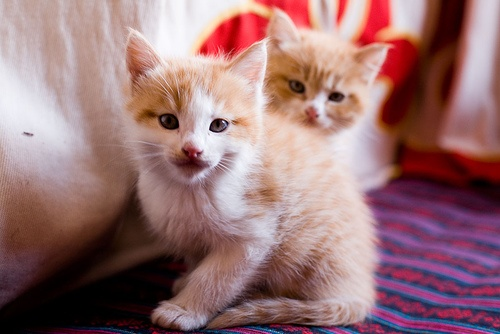
\includegraphics[width=8cm,height=8cm]{../examples/fcn8s/cats.jpg}};

\pic[shift={(1, 0, 0)}] at (0,0,0) 
    {Box={
        name=conv1,
        caption= ,
        xlabel={{3, }},
        zlabel=93,
        fill=\ConvColor,
        height=40,
        width=3,
        depth=45
        }
    };

\pic[shift={(10, 10, 0)}] at (0,0,0) 
    {Box={
        name=conv2_1,
        caption= ,
        xlabel={{9, }},
        zlabel=93,
        fill=\ConvColor,
        height=40,
        width=9,
        depth=45
        }
    };

\pic[shift={(10, -10, 0)}] at (0,0,0) 
    {Box={
        name=conv2_2,
        caption= ,
        xlabel={{3, }},
        zlabel=93,
        fill=\ConvColor,
        height=40,
        width=3,
        depth=45
        }
    };

\pic[shift={(18, 0, 0)}] at (0,0,0) 
    {Box={
        name=conv3,
        caption= ,
        xlabel={{3, 3, }},
        zlabel=93,
        fill=\ConvColor,
        height=40,
        width={4, 4},
        depth=45
        }
    };

\pic[shift={(25, 0, 0)}] at (0,0,0) 
    {Box={
        name=conv4,
        caption= ,
        xlabel={{3, 3, }},
        zlabel=93,
        fill=\ConvColor,
        height=40,
        width={4, 4},
        depth=45
        }
    };

\pic[shift={(30, 0, 0)}] at (0,0,0) 
    {Box={
        name=conv5,
        caption= ,
        xlabel={{3, 3, }},
        zlabel=93,
        fill=\ConvColor,
        height=40,
        width={2, 2},
        depth=45
        }
    };

\pic[shift={(35, 0, 0)}] at (0,0,0) 
    {Box={
        name=conv6,
        caption= ,
        xlabel={{3, 3, }},
        zlabel=93,
        fill=\ConvColor,
        height=40,
        width={2, 2},
        depth=45
        }
    };

\pic[shift={(40, 0, 0)}] at (0,0,0) 
    {Box={
        name=conv7,
        caption= ,
        xlabel={{3, 3, }},
        zlabel=93,
        fill=\ConvColor,
        height=40,
        width={2, 2},
        depth=45
        }
    };

\pic[shift={(45, 0, 0)}] at (0,0,0) 
    {Box={
        name=conv8,
        caption= ,
        xlabel={{3, 3, }},
        zlabel=93,
        fill=\ConvColor,
        height=40,
        width={2, 2},
        depth=45
        }
    };

\pic[shift={(50, 0, 0)}] at (0,0,0) 
    {Box={
        name=conv9,
        caption= ,
        xlabel={{3, 3, }},
        zlabel=93,
        fill=\ConvColor,
        height=40,
        width={2, 2},
        depth=45
        }
    };

\pic[shift={(55, 0, 0)}] at (0,0,0) 
    {Box={
        name=conv10,
        caption= ,
        xlabel={{3, }},
        zlabel=93,
        fill=\ConvColor,
        height=40,
        width=3,
        depth=45
        }
    };

\draw [connection]  (conv1-east)    -- node {\midarrow} (conv2_1-west);

\draw [connection]  (conv1-east)    -- node {\midarrow} (conv2_2-west);

\draw [connection]  (conv3-east)    -- node {\midarrow} (conv4-west);

\draw [connection]  (conv4-east)    -- node {\midarrow} (conv5-west);

\draw [connection]  (conv5-east)    -- node {\midarrow} (conv6-west);

\draw [connection]  (conv6-east)    -- node {\midarrow} (conv7-west);

\draw [connection]  (conv7-east)    -- node {\midarrow} (conv8-west);

\draw [connection]  (conv8-east)    -- node {\midarrow} (conv9-west);

\draw [connection]  (conv9-east)    -- node {\midarrow} (conv10-west);

\node (concatenate) at (14, 0, 0) {concatenate qconv};

\node (add) at (25, 10, 0) {add};

\node (add2) at (30, 10, 0) {add};

\node (add3) at (40, 10, 0) {add};

\node (add4) at (45, 10, 0) {add};

\node (concat1) at (35, 10, 0) {concatenate};

\node (concat2) at (50, 10, 0) {concatenate};

\draw[connection, to path={-| (\tikztotarget)}]
  (conv2_1-east) edge (concatenate) (concatenate) edge (conv3-west);

\draw[connection, to path={-| (\tikztotarget)}]
  (conv2_2-east) edge (concatenate) (concatenate) edge (conv3-west);

\draw[connection, to path={-| (\tikztotarget)}]
  (23, 0, 0) edge (add) (add) edge (27, 0, 0);

\draw[connection, to path={-| (\tikztotarget)}]
  (27.5, 0, 0) edge (add2) (add2) edge (32, 0, 0);

\draw[connection, to path={-| (\tikztotarget)}]
  (32, 0, 0) edge (concat1) (concat1) edge (36, 0, 0);

\draw[connection, to path={-| (\tikztotarget)}]
  (37.5, 0, 0) edge (add3) (add3) edge (39, 0, 0);

\draw[connection, to path={-| (\tikztotarget)}]
  (41.5, 0, 0) edge (add4) (add4) edge (43, 0, 0);

\draw[connection, to path={-| (\tikztotarget)}]
  (45, 0, 0) edge (concat2) (concat2) edge (48, 0, 0);


\end{tikzpicture}
\end{document}
